% Benchmark construction (top) and deployment of LOCUS in a digitisation pipeline (bottom). No numbers.
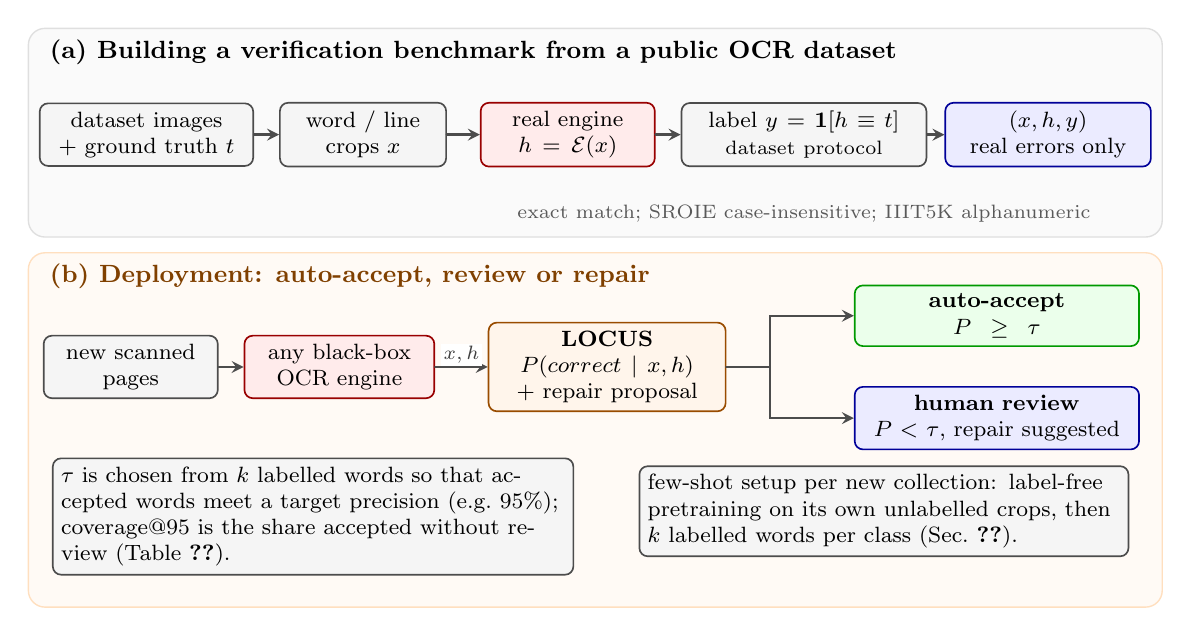
\begin{tikzpicture}[
  font=\small, >=stealth, line cap=round,
  box/.style={draw=#1!60!black, rounded corners=3pt, align=center, inner sep=3pt, fill=#1!8, line width=0.6pt, font=\footnotesize},
  box/.default=gray,
  flow/.style={->, line width=0.9pt, black!70},
  band/.style={rounded corners=6pt, fill=#1!4, draw=#1!25, line width=0.5pt},
  lbl/.style={font=\scriptsize\itshape, fill=white, inner sep=0.8pt, text=black!75},
]
\fill[band=gray]   (0,1.95) rectangle (14.4,4.6);
\fill[band=orange] (0,-2.75) rectangle (14.4,1.75);
\node[anchor=west, font=\small\bfseries] at (0.15,4.3) {(a) Building a verification benchmark from a public OCR dataset};
\node[anchor=west, font=\small\bfseries, text=orange!50!black] at (0.15,1.45) {(b) Deployment: auto-accept, review or repair};

% ---------------------------------------------------------------- (a)
\node[box, text width=2.5cm] (ds) at (1.5,3.25) {dataset images\\+ ground truth $t$};
\node[box, text width=1.9cm] (crop) at (4.25,3.25) {word / line\\crops $x$};
\node[box=red, text width=2.0cm] (eng) at (6.85,3.25) {real engine\\$h=\mathcal{E}(x)$};
\node[box, text width=2.9cm] (lab) at (9.85,3.25) {label $y=\mathbf{1}[h\equiv t]$\\{\scriptsize dataset protocol}};
\node[box=blue, text width=2.4cm] (bench) at (12.95,3.25) {$(x,h,y)$\\real errors only};
\draw[flow] (ds) -- (crop); \draw[flow] (crop) -- (eng); \draw[flow] (eng) -- (lab); \draw[flow] (lab) -- (bench);
\node[font=\scriptsize, text=black!65, align=center] at (9.85,2.25) {exact match; SROIE case-insensitive; IIIT5K alphanumeric};

% ---------------------------------------------------------------- (b)
\node[box, text width=2.0cm] (page) at (1.3,0.3) {new scanned\\pages};
\node[box=red, text width=2.2cm] (oc) at (3.95,0.3) {any black-box\\OCR engine};
\node[box=orange, text width=2.8cm] (lc) at (7.35,0.3) {\textbf{LOCUS}\\$P(\text{correct}\mid x,h)$\\+ repair proposal};
\draw[flow] (page) -- (oc); \draw[flow] (oc) -- node[lbl, above]{$x,h$} (lc);
\node[box=green, text width=3.4cm] (acc) at (12.3,0.95) {\textbf{auto-accept}\\$P\geq\tau$};
\node[box=blue, text width=3.4cm] (rev) at (12.3,-0.35) {\textbf{human review}\\$P<\tau$, repair suggested};
\draw[flow] (lc.east) -- ++(0.55,0) |- (acc.west);
\draw[flow] (lc.east) -- ++(0.55,0) |- (rev.west);
\node[box, text width=6.4cm, align=left, anchor=north west] at (0.3,-0.85)
  {$\tau$ is chosen from $k$ labelled words so that accepted words meet a target precision (e.g.\ 95\%);
   coverage@95 is the share accepted without review (Table~\ref{tab:review}).};
\node[box=gray, text width=6.0cm, align=left, anchor=north west] at (7.75,-0.95)
  {few-shot setup per new collection: label-free pretraining on its own unlabelled crops, then
   $k$ labelled words per class (Sec.~\ref{sec:pretrain}).};
\end{tikzpicture}
